\documentclass[UTF8,fontset=fandol,11pt,a4paper]{ctexart}
\usepackage[left=23mm,right=23mm,top=23mm,bottom=23mm,headheight=16pt]{geometry}
\usepackage{amsmath,amssymb,bm,mathtools,booktabs,graphicx,array,longtable,adjustbox}
\usepackage{xcolor,fancyhdr,caption,enumitem,needspace,xurl}
\usepackage[most]{tcolorbox}
\usepackage[colorlinks=true,linkcolor=blue!45!black,urlcolor=blue!45!black]{hyperref}
\newtcolorbox{resultbox}{breakable,colback=blue!3!white,colframe=blue!40!black,boxrule=.5pt,arc=1mm}
\newcommand{\ii}{\mathrm{i}}\newcommand{\dd}{\mathrm{d}}
\newcommand{\Rea}{\operatorname{Re}}\newcommand{\Ima}{\operatorname{Im}}
\numberwithin{equation}{section}
\setlength{\parskip}{3pt}\setlength{\emergencystretch}{3em}
\linespread{1.2}\allowdisplaybreaks[2]\raggedbottom
\pagestyle{fancy}\fancyhf{}
\fancyhead[L]{\small Kerr 标量散射：高精度与复响应}
\fancyhead[R]{\small 2026 年 10 月 23 日}
\fancyfoot[C]{\thepage}
\captionsetup{font=small,labelfont=bf}
\begin{document}
\begin{center}
{\LARGE\bfseries Kerr 标量场非线性散射研究增补笔记}\\[5mm]
{\large 极端频率、高精度谱方法与能流--相位约束}\\[3mm]
2026 年 10 月 23 日
\end{center}
\begin{resultbox}
本笔记收录 10 月 17 日 Overleaf 更新之后的研究：新径向谱仓库的审计、
$s=0$ 高精度推广、极低频与高频非线性重算，以及能流与相位不等式的证明和数值检验。
原论文的物理结果、图表和摘要保持原样；主线优化限于引言、极限之间的过渡和结论开头。
当前新数值单独存放，供审阅后决定论文中的整合方式。
\end{resultbox}
\setcounter{tocdepth}{1}
\tableofcontents\clearpage

\section{研究问题与证据层次}
固定 Kerr 背景上的局域自相互作用改变透射振幅的模和相位。
本轮问题是：当线性反射极小时，非线性能流修正如何与相位修正分离；
低频与高频数据能以多高精度检验同一复响应。
解析恒等式、有限参数的数值结果、待验证的渐近猜想分别陈述。

新仓库 \texttt{teukolsky-radial-spectral} 的审计版本为
\texttt{1621eb5e379b}（完整提交号保存在审计记录中）。
其主结果采用 $s=-2,\ell=m=2$；本笔记的非线性计算采用重新推导的 $s=0$ 方程。
本轮保留参考仓库原文件，标量实现位于 \path{src/kerr_scalar_precision.jl}。
Julia 1.10.7 运行时来自官方发行包，并核对官方 SHA256。

\section{统一约定与物理观测量}
取 $G=c=M=1$，度规号差为 $(-,+,+,+)$，时间与方位依赖为
$e^{-\ii\omega t+\ii m\phi}$。定义
\begin{gather}
r_\pm=1\pm\sqrt{1-a^2},\quad\Delta=(r-r_+)(r-r_-),\quad
K=(r^2+a^2)\omega-am,\\
\Omega_H=\frac{a}{2r_+},\quad p=\omega-m\Omega_H,\quad
\kappa=\frac{r_+-r_-}{4r_+},\quad \frac{\dd r_*}{\dd r}=\frac{r^2+a^2}{\Delta},\\
r_*=r+\frac{2r_+}{r_+-r_-}\ln\frac{r-r_+}{2}
-\frac{2r_-}{r_+-r_-}\ln\frac{r-r_-}{2}.
\end{gather}
该积分常数用于全部复振幅比较。
标量径向算子及角向常数为
\begin{equation}
\mathcal L R=(\Delta R')'+\left(\frac{K^2}{\Delta}-\lambda\right)R,
\qquad\lambda=A_{\ell m}+a^2\omega^2-2am\omega.
\end{equation}
角向函数按 $\int|S_{\ell m}|^2\dd\Omega=1$ 归一化。
视界与无穷远基底满足
\begin{gather}
I\sim e^{-\ii p r_*},\qquad D\sim r^{-1}e^{-\ii\omega r_*},\qquad
U\sim r^{-1}e^{\ii\omega r_*},\\
I=B^{\rm inc}D+B^{\rm ref}U,\qquad D=U^*\quad(\omega\in\mathbb R),\\
q=\frac{B^{\rm ref}}{B^{\rm inc}},\quad R^{(0)}=|q|^2,\quad
T^{(0)}=\frac{2r_+p}{\omega|B^{\rm inc}|^2},\quad T^{(0)}+R^{(0)}=1.
\end{gather}
对 $\Box\Phi+\epsilon_n|\Phi|^{2n}\Phi=0$，恢复 $M$ 后定义
$g_n=\epsilon_n/M^{2n-2}$ 与 $\eta=g_n|\mathcal A_{\rm in}|^{2n}$。
固定入射条件下
\begin{gather}
C_H=C_H^{(0)}[1+\eta\rho_n+O(\eta^2)],\\
\chi_n=2\Rea\rho_n,\quad\psi_n=\Ima\rho_n,\\
T/T^{(0)}=1+\eta\chi_n+O(\eta^2),\quad
\Delta\arg C_H=\eta\psi_n+O(\eta^2).
\end{gather}
表中的 $\chi_n,\psi_n$ 均为零耦合处的响应系数，物理改变量包含 $\eta$。

\section{从高精度三支谱法到标量实现}
\subsection{完整 Kerr 相位与精确消去}
引入 $\Psi'=K/\Delta$，显式积分得到
\begin{equation}
\Psi=\omega r_*-\frac{ma}{r_+-r_-}\ln\frac{r-r_+}{r-r_-}.
\end{equation}
为保持单位视界归一化，取
\begin{equation}
I=e^{-\ii(\Psi-C_H^{\rm ph})}Y,\qquad
C_H^{\rm ph}=\frac{ma}{2}+\frac{ma}{r_+}\ln\frac{r_+-r_-}{2},\qquad Y(r_+)=1.
\end{equation}
这里的 $C_H^{\rm ph}$ 是相位常数，与透射振幅 $C_H$ 分别定义。
将 $I$ 代回原始方程，$K^2/\Delta$ 项解析抵消，得到
\begin{equation}
\Delta Y''+(\Delta'-2\ii K)Y'+(-2\ii\omega r-\lambda)Y=0.
\end{equation}
无穷远两支写为 $R_\varsigma=r^{-1}e^{\varsigma\ii\Psi}u_\varsigma$，
$\varsigma=+1$ 对应 $U$，$\varsigma=-1$ 对应 $D$。对应包络方程为
\begin{align}
\Delta u''+b_\varsigma u'+c_\varsigma u&=0,\\
b_\varsigma&=\Delta'-2\Delta/r+2\varsigma\ii K,\\
c_\varsigma&=-2/r+2a^2/r^2-\lambda
+2\varsigma\ii(am-a^2\omega)/r.
\end{align}
这些系数由标量算子重新得到，保留 $m$ 的显式依赖。

\subsection{紧化、端点与整体匹配}
令 $z=r_+/r$，则 $z_r=-z^2/r_+$，$z_{rr}=2z^3/r_+^2$，
\begin{equation}
B_2=\Delta z_r^2,\qquad B_1=\Delta z_{rr}+b z_r,\qquad B_0=c.
\end{equation}
视界和无穷远都有 $B_2=0$，通过 $B_1u_z+B_0u=0$ 与 $u=1$ 固定端点。
对无穷远新相位约定，$B_1(0)=-2\varsigma\ii\omega r_+$，$B_0(0)=-\lambda$。
视界支的 $B_1(1)=-(r_+-r_--2\ii K_+)/r_+$。
每个有限子域使用 Chebyshev--Lobatto 节点，接口施加函数及一阶导数连续性。
所有单元联立求解，端点属于谱网格。

有限单元按 $2\omega|\Delta r_*|$ 的相位跨度分割；低频无穷远首单元宽度取
$z_0=\min(0.025,\omega r_+/20)$，随后采用几何分域。
内外区和三支基底的谱阶可以分别指定。
工作位数控制舍入，谱阶和分域控制离散误差，两者分别加密。

\subsection{高精度线性系统与振幅提取}
行列均衡后的系统为 $Ax=b$。双精度 LU 提供近似求解器，
残差在 BigFloat 中计算：
\begin{equation}
r_k=b-Ax_k,\qquad x_{k+1}=x_k+\widetilde A^{-1}r_k.
\end{equation}
接受条件使用高精度后向误差
$\|r_k\|_\infty/(\|A\|_\infty\|x_k\|_\infty+\|b\|_\infty)$。
迭代收敛依赖预条件近似的有效性，脚本记录失败状态。
在重叠区提取
\begin{equation}
B^{\rm ref}=\frac{DI'-D'I}{DU'-D'U},\qquad
B^{\rm inc}=\frac{IU'-I'U}{DU'-D'U}.
\end{equation}
分子相消比衡量微小反射的位数损失。五个匹配半径分别检查振幅稳定性。
相对原方程残差使用
\begin{equation}
\delta_{\mathcal L}=\frac{|\Delta R''+\Delta'R'+VR|}
{|\Delta R''|+|\Delta'R'|+|VR|},\qquad V=K^2/\Delta-\lambda.
\end{equation}
分母包含场本身，使指标保持归一化不变性。

\section{非线性投影的高精度积分}
自耦合通道的正权重为
\begin{equation}
P_n=r^2C_0^{(n)}+a^2C_2^{(n)},\qquad
C_j^{(n)}=\int (\cos\theta)^j|S|^{2n+2}\dd\Omega\quad(j=0,2).
\end{equation}
固定入射场 $F=I/B^{\rm inc}$ 直接消去源的巨大归一化因子。
定义
\begin{equation}
J_d=\int P_n|F|^{2n}|U|^2\dd r,\qquad
J_o=\int P_n|F|^{2n}U^2\dd r.
\end{equation}
则 $\rho_n=\ii(J_d+qJ_o)/(2\omega)$，此处取 $M=1$。
对一般 $M$，右侧还包含 $M^{2n-2}$。

视界侧在 $t=\ln[(r-r_+)/(r_+-r_-)]$ 上分段 Gauss 积分，
视界遗漏的小区间使用领先幂函数的解析积分。数值实现中的截点属于积分规则，
径向谱方程的边界仍位于精确视界。
无穷远侧利用 $F=D+qU$ 展开
\begin{equation}
|F|^2=(1+|q|^2)DU+qU^2+q^*D^2.
\end{equation}
$n$ 次幂形成有限个相位通道 $e^{2\ii j\Psi}$。
非振荡通道用 Gauss 积分；振荡通道通过 Levin 辅助方程
\begin{equation}
v_z+2\ii j\Psi_z v=f(z)
\end{equation}
转化为包络谱求解。乘以 $z^2$ 后在紧化无穷远施加正则条件，积分由端点值读出。
对极小 $J_o$，视界侧与无穷远侧还存在相消，接受精度由独立加密的响应变化衡量。
本实现由同一分解计算 $R^{(1)}$，相应能流平衡属于代数检查；
独立证据来自原方程残差、谱尾、匹配位置及积分加密。
最新积分实现对一阶辅助方程逐单元前代，保持相同配点方程和连续性条件，
将辅助矩阵的存储量限制在单个单元。两次内存保护终止的记录及各版源码均保留。
另一次启动脚本哈希发生变化的运行保留为输入变更记录，并以新目录重算；
汇总表只纳入输入前后哈希一致的成功运行。
极小线性反射率由 $|B^{\rm ref}/B^{\rm inc}|^2$ 直接计算；
接近一的透射率需要单独报告其绝对误差和微小反射通道的相对误差。

\section{能流--相位不等式的完整推导}
\subsection{正权重与响应圆盘}
由于 $P_n|F|^{2n}\geq0$ 且 $|U^2|=|U|^2$，三角不等式给出
\begin{equation}
|J_o|\leq J_d.
\end{equation}
令 $D_n=J_d/(2\omega)>0$、$z_n=qJ_o/J_d=x+\ii y$、$r=|q|$，则
\begin{gather}
|z_n|\leq r,\qquad\rho_n=\ii D_n(1+z_n),\\
\chi_n=-2D_ny,\qquad\psi_n=D_n(1+x),\\
\left(\frac{\chi_n}{2}\right)^2+(\psi_n-D_n)^2\leq D_n^2r^2.
\end{gather}
这是复响应在平面中的圆盘约束。

\subsection{消去源积分后的可观测约束}
在 $\omega>0,p>0$ 的非超辐射区，$0\leq r<1$，从而 $\psi_n>0$。
最大化
\begin{equation}
\frac{y^2}{(1+x)^2}\leq\frac{r^2-x^2}{(1+x)^2}
\end{equation}
时，极值位于 $x=-r^2$，并得到
\begin{resultbox}
\begin{equation}
\boxed{\frac{|\chi_n|}{2\psi_n}\leq\frac{r}{\sqrt{1-r^2}}
=\sqrt{\frac{R^{(0)}}{T^{(0)}}}.}
\end{equation}
适用条件：实正频率、$p>0$、实局域耦合、固定入射归一化、正权重自耦合通道，
且相应 Green 积分收敛。一般 $M$ 的正比例因子在该比值中抵消。
\end{resultbox}
等号还要求积分三角不等式饱和，并满足圆盘切线条件；一般散射解保留严格余量。
对 $p<0$，$r>1$，上述圆盘仍成立，关于 $\psi_n$ 符号及比值的结论需要另行分析。
阈值 $p=0$ 对应 $T^{(0)}=0$，分式界应以适当极限处理。

\subsection{与能流零点及高频的关系}
$\chi_n=0$ 的条件为 $\Ima(qJ_o)=0$，同时 $\psi_n$ 可保持有限。
在 $R^{(0)}\to0$ 的参数序列上，不等式给出
$|\chi_n|/\psi_n=O(\sqrt{R^{(0)}})$ 的上界。
这是相对相位占优的约束，绝对相位大小仍由 $J_d$ 决定。
近极端 principal 模态的 $\sigma^{-n}$ 增强控制响应整体尺度，
该圆盘约束控制实部与虚部的相对大小，两者提供互补信息。
现有 27 个精细相位样本均满足该界，最大饱和比约为 $0.622$。
新极低频和高频样本的检验列于下一节。
本轮 $a=0.5,\ell=m=0,n=3$ 的极低频响应为正，$\omega=3$ 的响应为负。
在该实频区间上响应连续的条件下，中间值定理保证至少一个能流零点。
其精确位置、零点数量与相位值需要在该区间进一步定位和加密。

\section{本轮新计算与收敛}
配对接受门槛分别为 $|\chi_{\rm fine}/\chi_{\rm coarse}-1|<10^{-8}$、
$|\rho_{\rm fine}/\rho_{\rm coarse}-1|<10^{-10}$，
原方程残差小于 $10^{-25}$，谱尾小于 $10^{-20}$，
五点匹配的反射振幅相对展宽小于 $10^{-8}$，线性能流平衡误差小于 $10^{-25}$。
同时检查 $|J_o|\leq J_d$、相位正性与能流--相位约束。
在 $\ell=0,\omega=0.1$ 和 $\ell=2,\omega=10^{-5}$ 上另行固定径向设置、
提高积分阶数；后者相位的相对变化约为 $10^{-65}$。
粗细配对中径向位数、谱阶和积分阶数共同提高，独立积分检验补充了单独误差来源的检查。
\subsection{参数、精度与证据范围}
新计算统一采用 $a=0.5$、固定入射归一化。粗细两档分别使用 320/384 bit，
内区阶数 64/80、外区阶数 48/64，积分阶数和 Levin 阶数独立提高。
当前共有 21 个配对参数点，其中 21 个通过预设接受门槛。
表中数字展示物理尺度；完整有效数字及逐项误差保存在 CSV 和 TOML 中。
\begin{longtable}{rrrrrr}
\caption{新标量非线性散射结果。$m=0$；$\mathcal S=|\chi|/[2\psi\sqrt{R^{(0)}/(1-R^{(0)})}]$。}\\
\toprule $\ell$ & $n$ & $\omega$ & $\chi_n$ & $\psi_n$ & $\mathcal S$\\\midrule\endfirsthead
\toprule $\ell$ & $n$ & $\omega$ & $\chi_n$ & $\psi_n$ & $\mathcal S$\\\midrule\endhead
0 & 1 & $1.0\times10^{-5}$ & $0.2206456$ & $0.2500066$ & $1.71\times10^{-5}$\\
0 & 2 & $1.0\times10^{-5}$ & $6.317813\times10^{-12}$ & $3.979159\times10^{-12}$ & $3.07\times10^{-5}$\\
0 & 3 & $1.0\times10^{-5}$ & $1.72461\times10^{-22}$ & $8.444427\times10^{-23}$ & $3.95\times10^{-5}$\\
1 & 1 & $1.0\times10^{-5}$ & $0.1471387$ & $0.2100021$ & $3.91\times10^{-11}$\\
2 & 1 & $1.0\times10^{-5}$ & $0.1063674$ & $0.1683684$ & $4.07\times10^{-17}$\\
0 & 1 & $1.0\times10^{-4}$ & $0.2207357$ & $0.2500659$ & $1.71\times10^{-4}$\\
1 & 1 & $1.0\times10^{-4}$ & $0.1471567$ & $0.2100212$ & $3.91\times10^{-9}$\\
2 & 1 & $1.0\times10^{-4}$ & $0.1063751$ & $0.1683779$ & $4.07\times10^{-14}$\\
0 & 1 & $1.0$ & $1.112854\times10^{-11}$ & $0.02087919$ & $3.56\times10^{-5}$\\
0 & 1 & $2.0$ & $6.401732\times10^{-23}$ & $0.01045553$ & $1.4\times10^{-10}$\\
0 & 1 & $3.0$ & $5.497823\times10^{-34}$ & $0.007311307$ & $5.26\times10^{-16}$\\
0 & 2 & $3.0$ & $1.551077\times10^{-35}$ & $5.889127\times10^{-5}$ & $1.84\times10^{-15}$\\
0 & 3 & $3.0$ & $-1.969823\times10^{-36}$ & $9.020307\times10^{-7}$ & $1.53\times10^{-14}$\\
1 & 1 & $3.0$ & $3.733594\times10^{-33}$ & $0.01392532$ & $9.53\times10^{-16}$\\
2 & 1 & $3.0$ & $8.793907\times10^{-32}$ & $0.01405412$ & $4.24\times10^{-15}$\\
0 & 1 & $5.0$ & $6.450157\times10^{-56}$ & $0.006337859$ & $6.56\times10^{-27}$\\
0 & 2 & $5.0$ & $2.326749\times10^{-57}$ & $9.093391\times10^{-5}$ & $1.65\times10^{-26}$\\
0 & 3 & $5.0$ & $-1.578132\times10^{-57}$ & $2.685534\times10^{-6}$ & $3.79\times10^{-25}$\\
0 & 1 & $10.0$ & $5.493329\times10^{-111}$ & $0.009108419$ & $1.75\times10^{-54}$\\
0 & 2 & $10.0$ & $9.421642\times10^{-113}$ & $3.836582\times10^{-4}$ & $7.13\times10^{-55}$\\
0 & 3 & $10.0$ & $-2.429499\times10^{-111}$ & $3.257994\times10^{-5}$ & $2.17\times10^{-52}$\\
\bottomrule\end{longtable}
\subsection{数值质量}
最大配对能流响应变化为 $1.362964\times10^{-19}$，
最大配对相位变化为 $1.478465\times10^{-40}$。
最高采样径向残差为 $4.514484\times10^{-62}$。
最大谱尾指标为 $5.211527\times10^{-61}$，
五点匹配半径下的最大反射振幅相对展宽为 $3.896329\times10^{-47}$。
成功配对运行记录中的最大进程峰值内存约为 1314 MB。
该组精度陈述对应独立加密的一致性和离节点原方程检查；外部高精度标量参考列为待完成检验。
\begin{figure}[htbp]\centering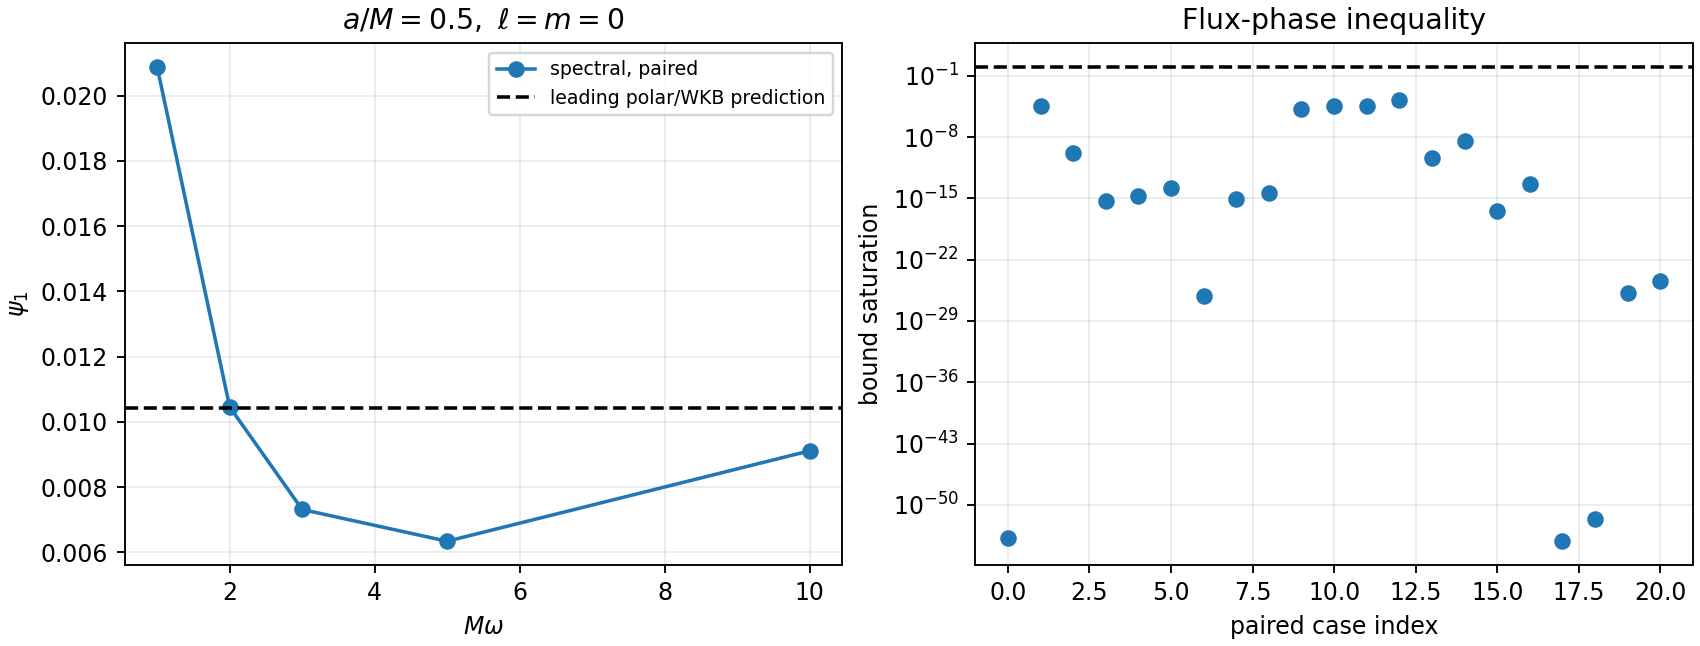
\includegraphics[width=.98\textwidth]{../../results/precision_20261023/response_summary.png}
\caption{新高精度标量结果。左：单极子三次响应的相位系数；右：各已配对点的不等式饱和比。}\end{figure}

\subsection{最高频点的振荡相消}
在 $a=0.5,\ell=m=0,n=1,\omega=10$，完整配对计算得到
\begin{gather}
R^{(0)}=2.96352916\times10^{-110},\qquad
\chi_1=5.49332942\times10^{-111},\\
\psi_1=9.10841931\times10^{-3},\qquad
|J_o|/J_d=1.81617660\times10^{-54}.
\end{gather}
该点的不等式饱和比为 $1.75169\times10^{-54}$，
且 $\chi_1/R^{(0)}=0.18536445$。
线性反射与源积分的振荡相消共同抑制能流实部，相位由正定积分 $J_d$ 主导。
通用圆盘约束在该频点保留很大的余量。
判断 $\chi_1/R^{(0)}$ 的渐近行为需要连续频率扫描及独立积分加密；
上述比值作为有限频率数值结果记录。

\section{高频衰减尺度的可检验问题}
新参考仓库的 $s=-2$ 振幅在 $M\omega=3$ 至 10 下降约 39.32 个数量级。
对数曲线具有可解析的平滑曲率，局部振幅衰减率先增后减。
加入代数前因子后的指数参数对窗口敏感。该事实给标量研究提供了明确检验：
分别求线性反射、非线性振荡积分与相位，再组合成能流修正。
一般情况下，能流尾部指数同时受两个复量及其干涉控制。
本轮标量新数据保持与旧稿的有限窗口拟合分开，待连续频率扫描及误差门槛完成后更新渐近结论。

\section{高频角向局域化与相位的领先预测}
\subsection{单极子角向方程的局部极限}
对固定 $a>0$ 的 $(\ell,m)=(0,0)$ 模态，取 $c=a\omega\gg1$。
大实频率角向展开的系统背景见 Casals、Ottewill 与 Warburton 的研究\cite{Casals2019}。
角向方程在北极 $\theta\ll1$ 处化为
\begin{equation}
S_{\theta\theta}+\theta^{-1}S_\theta+
[A+c^2-c^2\theta^2]S=0.
\end{equation}
领先基态满足 $A=-c^2+2c+O(1)$、
$S\simeq\mathcal N e^{-c\theta^2/2}$。
南北两极贡献相等，单位角向归一化要求
\begin{equation}
2\times2\pi\mathcal N^2\int_0^\infty\theta e^{-c\theta^2}\dd\theta=1,
\qquad\mathcal N^2=\frac{c}{2\pi}.
\end{equation}
由此
\begin{equation}
C_0^{(n)}\sim\frac{c^n}{(2\pi)^n(n+1)},\qquad
\frac{C_2^{(n)}}{C_0^{(n)}}\to1.
\end{equation}
高频极限中的角向积分具有非平凡频率依赖。

\subsection{径向 WKB 与非线性相位}
采用固定入射振幅和固定次极端自旋，领先传播波满足
\begin{equation}
|U|^2\sim|F|^2\sim\frac1{r^2+a^2},\qquad q\to0.
\end{equation}
在该 WKB 近似对源积分有效、且领先项允许逐项积分的条件下，
\begin{equation}
\psi_n\sim\frac{a^n\omega^{n-1}}{2(2\pi)^n(n+1)}
\mathcal I_n(a),\qquad
\mathcal I_n(a)=\int_{r_+}^\infty\frac{\dd r}{(r^2+a^2)^n}.
\end{equation}
因此领先预测为 $\psi_1\to\mathrm{const}$、$\psi_2\propto\omega$、
$\psi_3\propto\omega^2$。这些结论同时使用角向局域化和径向传播近似。
积分由
\begin{gather}
\mathcal I_1=\frac1a\arctan\frac a{r_+},\\
\mathcal I_n=\frac{2n-3}{2(n-1)a^2}\mathcal I_{n-1}
-\frac{r_+}{2(n-1)a^2(r_+^2+a^2)^{n-1}}
\end{gather}
计算。三次相互作用的单极子给出
\begin{equation}
\boxed{\psi_1\longrightarrow\frac1{8\pi}\arctan\frac a{r_+}.}
\end{equation}
在 $a=0.5$ 时，这个领先值为 $1/96$。
当前完整计算用于检验向该值靠近的趋势，有限窗口上的回升与极限值的证明分别表述。
为区分有限 $a\omega$ 的角向修正与径向传播修正，还计算
\begin{equation}
\psi_n^{\rm ang+WKB}=\frac{C_0^{(n)}\mathcal I_n+
a^2(C_2^{(n)}-C_0^{(n)})\mathcal I_{n+1}}{2\omega}.
\end{equation}
该表达式保留数值角向积分，在径向使用领先 WKB 场。
\begin{table}[htbp]\centering
\caption{$\omega=10$ 的完整谱相位与精确角积分加领先径向 WKB。}
\begin{tabular}{rrrr}\toprule $n$ & $\psi_n$ & $\psi_n^{\rm ang+WKB}$ & 相对差\\\midrule
1 & $0.009108419$ & $0.009089741$ & $0.002050648$\\
2 & $3.836582\times10^{-4}$ & $3.822473\times10^{-4}$ & $0.003677636$\\
3 & $3.257994\times10^{-5}$ & $3.243753\times10^{-5}$ & $0.004371112$\\
\bottomrule\end{tabular}\end{table}
角向独立检查取 $n=1,2,3$，频率依次为 $\omega=1,2,3,5$ 及 $10,20,50,100$。
球谐截断从 48 提至 64，最高两个频率从 96 提至 112；
角向积分最大相对变化为 $9.567642\times10^{-38}$。
$\omega=100$ 时，三个 $C_0^{(n)}$ 与领先极区近似之比分别为 $0.98987,0.97986,0.96996$。
该延伸检查仅计算角向问题；完整径向非线性结果的最高频率为 $\omega=10$。

固定 $a=0$ 时角向函数保持球谐形式，相应领先相位为 $O(\omega^{-1})$；
$a\omega\gg1$ 的展开对 $a\to0$ 具有非均匀性。

若改为固定入射能流，则 $|\mathcal A_{\rm in}|^2\propto\omega^{-2}$，
物理相位修正的上述领先估计变为 $\eta\psi_n\propto\omega^{-n-1}$。
频率增长时响应系数的幂律与具体照明条件共同决定物理改变量。

\section{有限耦合与波包的解释边界}
若 $C/C_0=1+\eta\rho_1+\eta^2\rho_2+\cdots$，则二阶能流包含
\begin{equation}
|\rho_1|^2+2\Rea\rho_2.
\end{equation}
首阶能流零点处的有限耦合预测需要二阶受迫场及新增角通道的能流。
视界相位用于描述传输响应；外部观测量需要反射相位或波包时延。
若脉冲持续时间满足 $\tau\propto\kappa^{-1}$，固定总入射能量使功率正比于 $\kappa$；
这一条件估计可以补偿定态 $\kappa^{-n}$ 增强的实幂因子。
定量波包计算需要处理 $|\Phi|^{2n}\Phi$ 的频率卷积。

\section{原稿主线审阅与此次修改边界}
原稿包含有限频率谱、固定自旋红外极限、近极端固定失谐极限。
三组计算共用固定入射的复 Green 响应，物理控制机制依次为源加权共振、
穿透因子的消去和喉区场浓集。
原有过渡段对这个共同对象强调偏弱，读者容易把三组结果读作独立主题。
此次在引言明确共同响应，在两种极限之间说明控制参数的改变，在结论开头回收同一逻辑。
摘要、全部 154 个显示公式及表图环境均保持逐字一致；所有旧数值与图文件保持原样。
新数值和本轮不等式单独进入本笔记，供审阅。

\section{复现与后续检验}
方程与角向测试入口为 \path{scripts/test_scalar_precision_20261023.jl}。
当前 192 项 Julia 检查和 33 项既有 Python 单元测试通过。
有界运行入口为 \path{scripts/run_scalar_precision_campaign_20261023.py}。
每个实验目录记录命令、输入前后 SHA256、输出 SHA256、运行时、内存峰值与参数。
完整数字存放在 \path{results/precision_20261023/}。
复算使用新的实验目录名，原结果保留。
后续优先增加同一频率的独立积分表示、角向截断加密，以及高频连续扫描。
对最低频的全局能流和最高频的微小源投影，分别检验其相消预算。
\begin{thebibliography}{9}
\bibitem{Casals2019} M. Casals, A. C. Ottewill, and N. Warburton,
High-order asymptotics for the spin-weighted spheroidal equation at large real frequency,
Proc. R. Soc. A \textbf{475}, 20180701 (2019),
\href{https://doi.org/10.1098/rspa.2018.0701}{doi:10.1098/rspa.2018.0701}.
\bibitem{SpectralRepo} Jing-Qi Lai, \texttt{teukolsky-radial-spectral},
\href{https://github.com/ljq2088/teukolsky-radial-spectral}{私人研究仓库}，
本轮审计版本 \texttt{1621eb5e379b}，2026 年 10 月 21 日。
\end{thebibliography}
\end{document}
